\chapter{Design}
\label{cha:design}
Implementing a simulation of a given system brings up different design questions regarding complexity of modules and the designed hierarchy.

\section{Modular design}
\label{sec:design_modular}
Designing a modular system in OMNeT++ with a bigger number of modules connected with channels and grouped in compound modules allows a more dynamic simulation and can increase the reuse-ability of modules.
This approach is convenient for simulating deep features and procedures within systems.
When a simulated system or network consists of multiple systems such a design can be problematic in sight of communication and simulation overhead.
Approaching emulation and the field of \emph{HiL} using the real time simulation these design decisions are important for the achieved timings.

A example of a modular design is shown in figure \ref{fig:OMNeTModularDesign}.

\begin{figure}
    \centering
    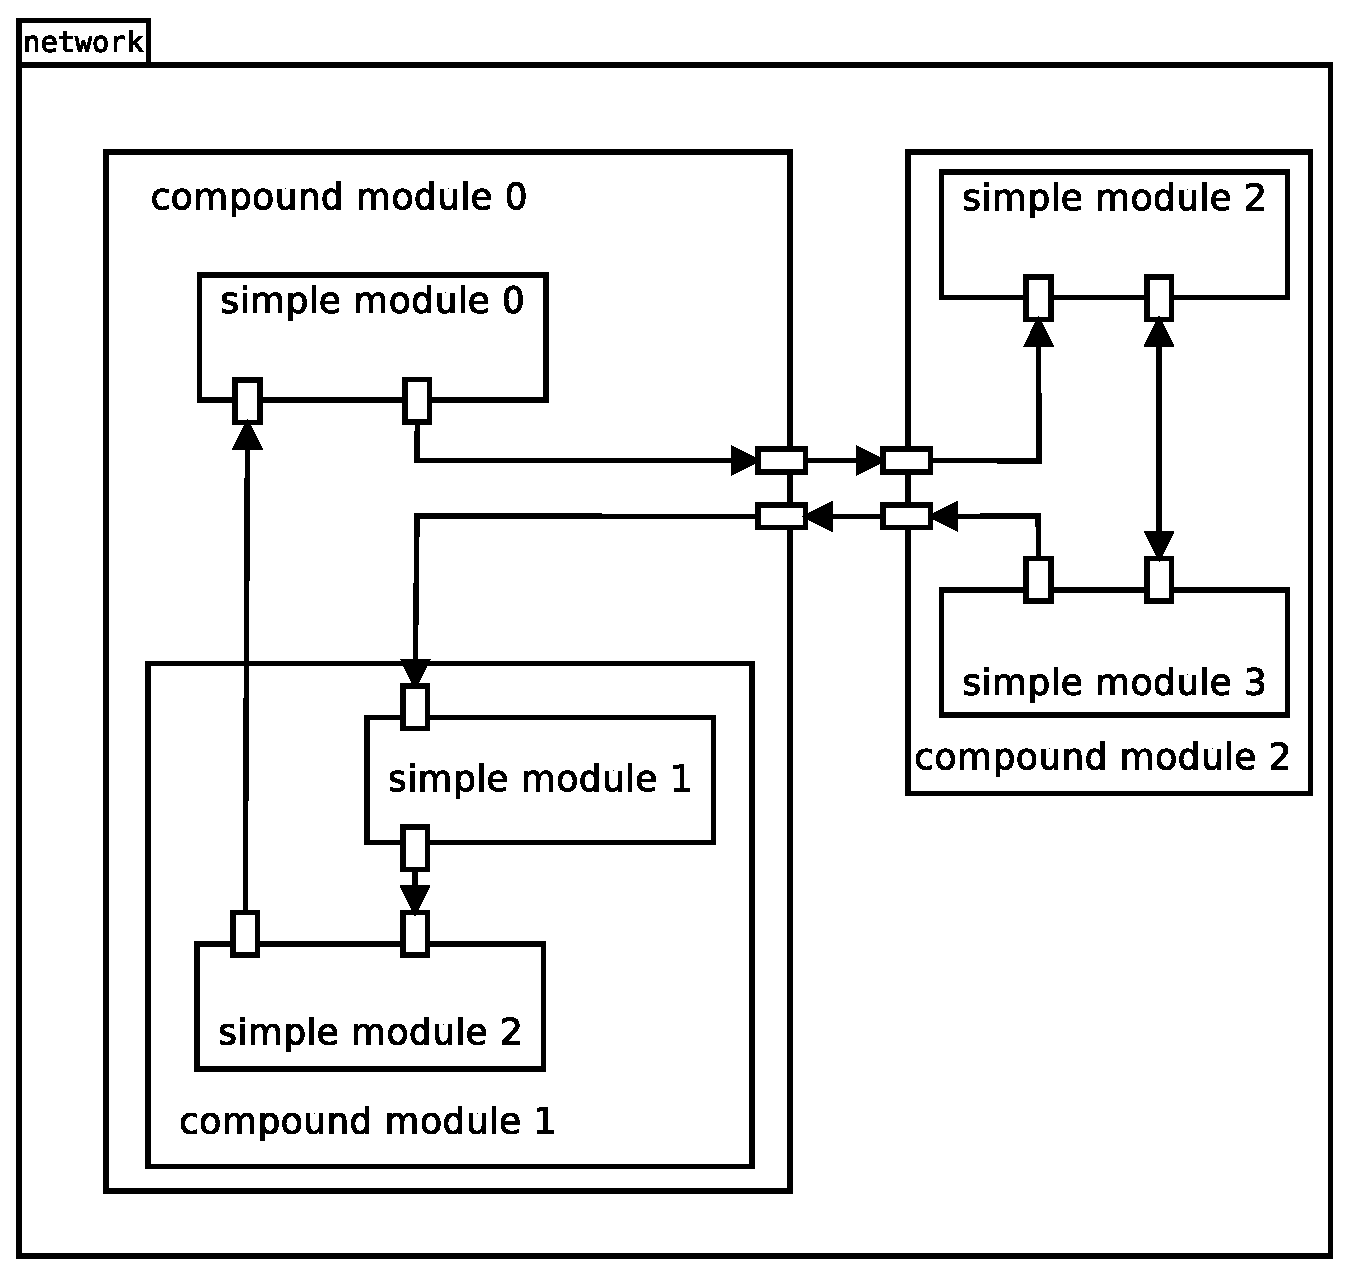
\includegraphics[width=0.9\columnwidth]{OMNeTModularDesign.eps}
    \caption{Modular design with OMNeT++}
    \label{fig:OMNeTModularDesign}
\end{figure}

As described in \cite[2.8]{varga_overview_2008} OMNeT++ provides functionalities for running a parallelized simulation and therefore increase the performance by parallelism.
A key requirement for parallelization of an OMNeT++ simulation is the modularization and the communication with messages and channels.
Different modules communicating with each other via messages sent over channels, as recommended in the User Guide \cite{omnet_manual}, can be executed on different logical processors.
The transmitted messages will be transmitted by a definable method, for example pipes, or a MPI (message passing interface).
Strongly depending on the simulated system this parallelization can result in an improvement of the execution speed and therefore improve the capabilities of real time simulation.

The implementation of a modular design is only possible if the simulated system, e.g. an existing application, is design modular.
I.e. different modules/classes communicate with each other via interfaces, function pointer etc..
If this requirement is met, these communication parts can be used for redirecting calls to the implementation of wrapper modules.
These modules build OMNeT++ messages from returning calls, decapsulate transmitted parameter from received messages and forward the calls to the enclosing modules.

\section{Monolithic design}
\label{sec:design_monolithic}
Decreasing the overhead of communication and simulation can be achieved for example by condensing a compound module to a simple module with more complex functions to execute.
This leads to a monolithic design containing less modules with more complex functions.
The execution of the single modules include more normal C++ code using simple method calls and operations.

The previous example network showing a modular design in figure \ref{fig:OMNeTModularDesign} can be condensed to a more monolithic design.
In the example, shown in figure \ref{fig:OMNeTMonolithicDesign}, the compound modules 0 and 2 with all their submodules were replaced by two simple modules.
The channels and the sent messages between the modules stay the same, but the calculation within the modules include the complete behavior of the previously included components.

\begin{figure}
    \centering
    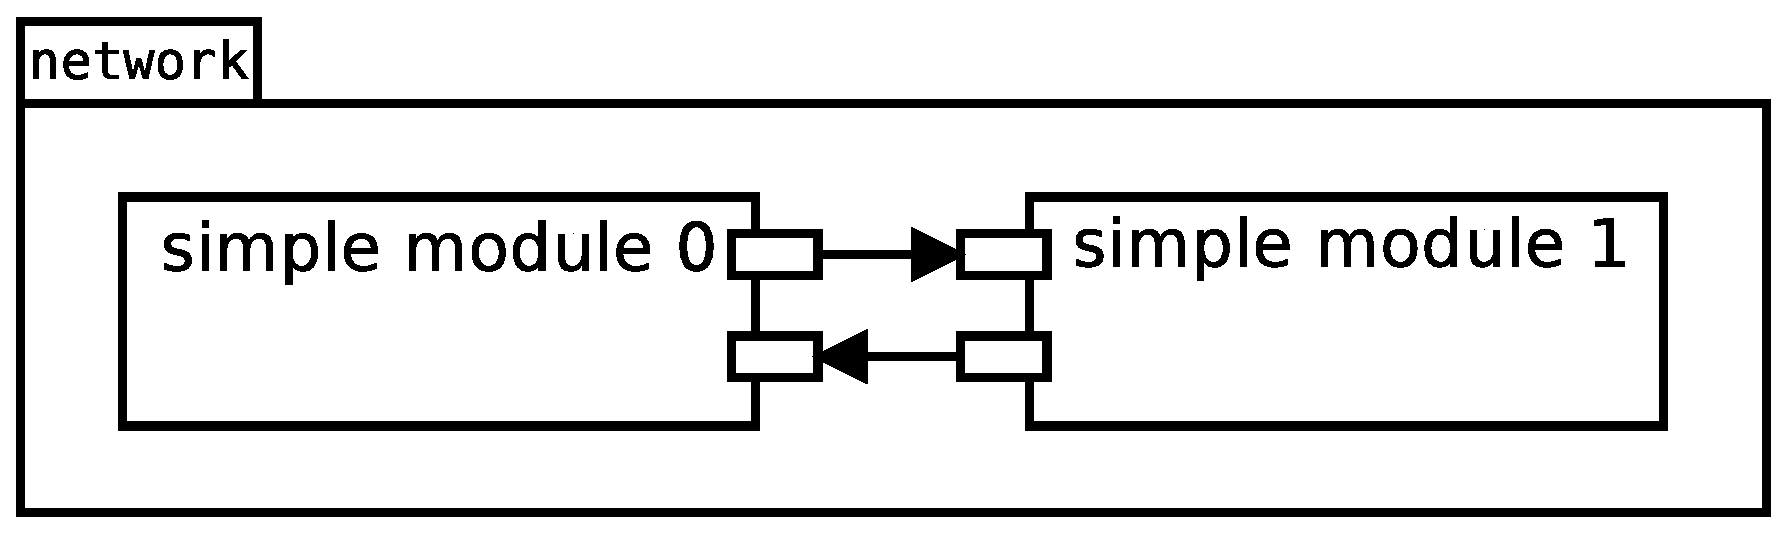
\includegraphics[width=0.9\columnwidth]{OMNeTMonolithicDesign.eps}
    \caption{Monolithic design with OMNeT++}
    \label{fig:OMNeTMonolithicDesign}
\end{figure}

